\documentclass[twoside]{protokoll}
\usepackage{graphicx}
\usepackage{tabularx} % for better table formatting
\usepackage{booktabs} % for better table formatting
\usepackage{float} 
\praktikum{I}
\usepackage{subfig}
\usepackage{amsmath}

\versuchsgebiet{(Akustik)}


\teilnehmer{Maximilian Carlos Menke, 434170}
\teilnehmer{Andrea Roth, 428396}
\gruppe{A3}

\begin{document}
 

%\begin{figure}[H]
%  \centering
%  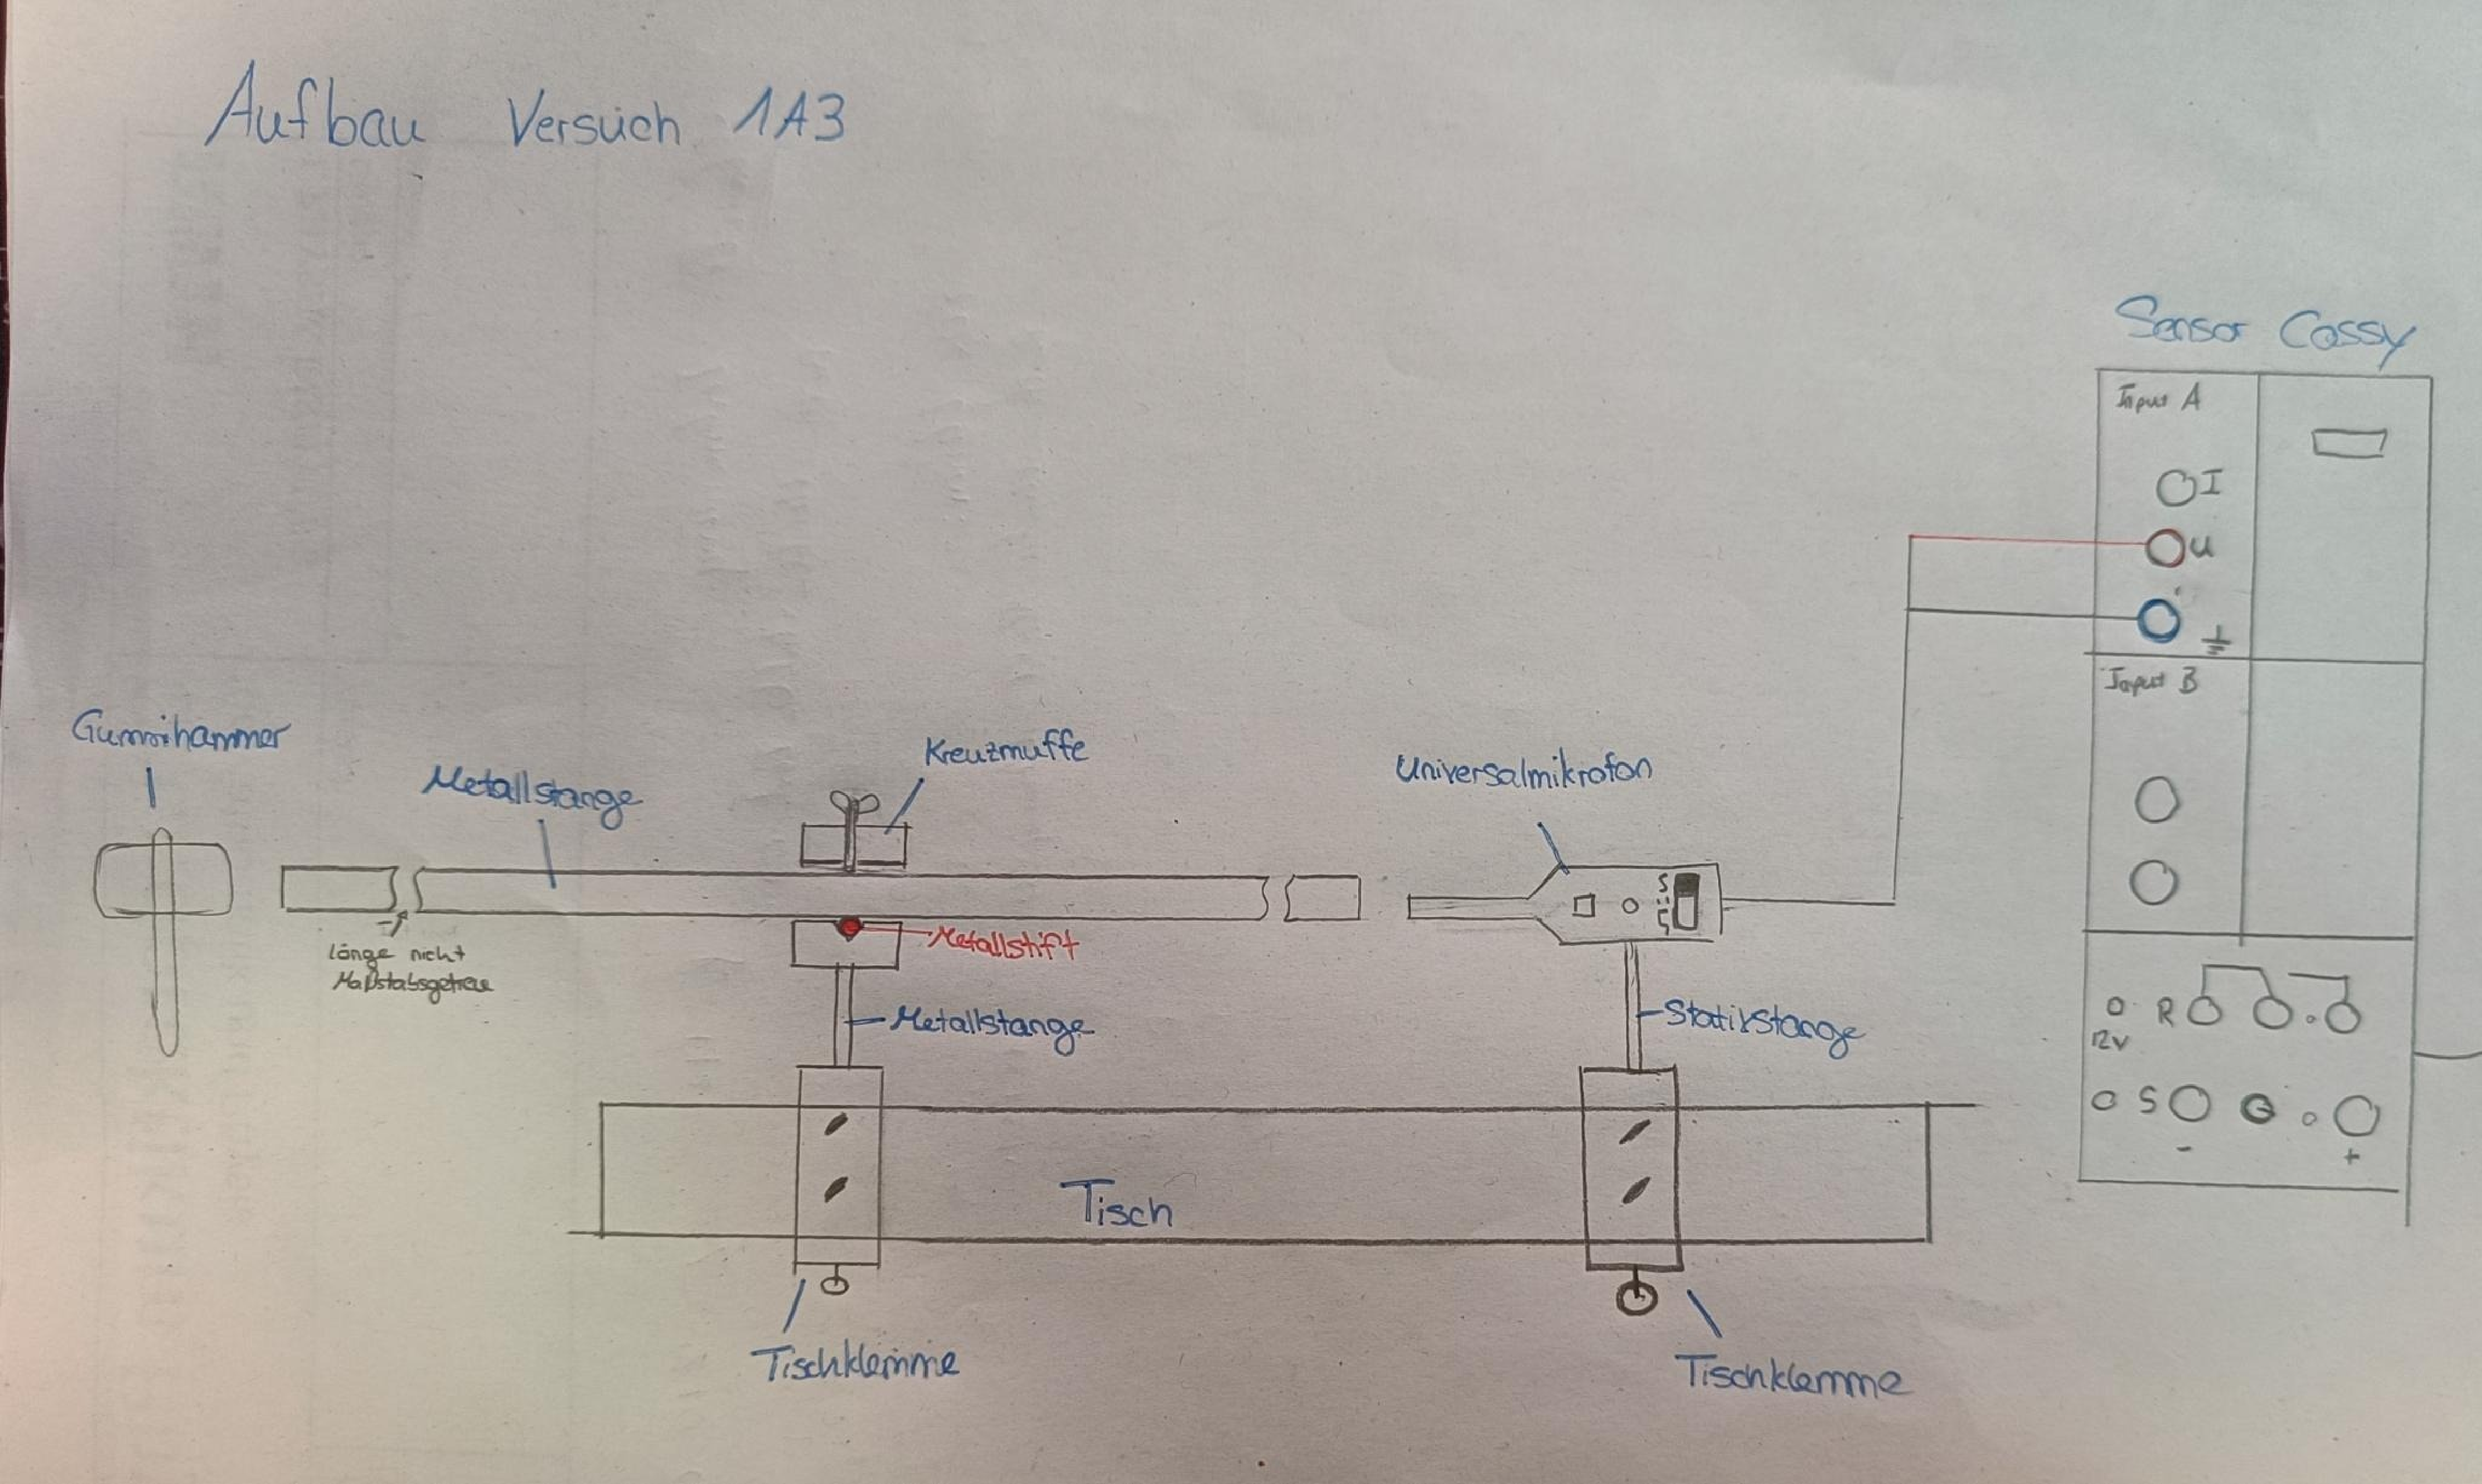
\includegraphics[width=1\textwidth]{Bilder/434170_428396_1A3_SkizzeAufbau.pdf}
%  \caption{Skizze des Versuchsaufbaus}
%  \centering
%\end{figure}



 

\begin{versuchsziele}
\end{versuchsziele}

\section{1E1 Ladekurven eines Kondensators}


\begin{versuchsziele}
Ziel des Versuchs ist die Kapazität eines Kondensators durch lade und entladevorgang
zu bestimmen. 
Dieser wird durch eine Schaltung mit Wiederstand und Schalter bestimmt.
Hierfür werden verschiedene Methoden verwendet. Mit dem Multimeter werden Kapazität
und Wiederstand bestimmt.
Mit dem Osziloskop wird die Kapazität bestimmt. Und mit Sensor CASSY 2 zunächst der 
Wiederstand 
\end{versuchsziele}


\begin{aufgabe}{Grundlagen}
  Knappe Beschreibung der theoretischen Grundlagen, Angabe der
  benötigten Formel(n), ohne Herleitung. Definition der verwendeten
  Formelzeichen.
\end{aufgabe}

% Bitte belassen Sie die Aufgabentexte in Ihrem Protokoll und beginnen
% Sie hier mit der Lösung der ersten Aufgabe:



\begin{aufgabe}{Vorversuch: Charakterisierung der verwendeten Bauteile}
  Charakterisieren Sie die verwendeten Bauteile mit Digitalvoltmeter
  und Messbrücke.
\end{aufgabe}


\begin{aufgabe}{Vorversuch: Bestimmung des Ohmschen Widerstands}
  Beschreiben Sie den Versuchsaufbau unter Verwendung eines
  Schaltbildes. Beschreiben Sie die Versuchsdurchführung unter Angabe
  der relevanten Messwerterfassungseinstellungen. Zeigen Sie
  exemplarisch die Häufigkeitsverteilungen für Spannung $U$ und Strom
  $I$ an einem Messpunkt und beschreiben Sie, wie Sie die
  statistischen Fehler für $U$ und $I$ bestimmen. Tragen Sie die
  Spannung $U$ gegen den Strom $I$ auf und bestimmen Sie aus der
  Steigung den Widerstand $R$ und seine statistische
  Messunsicherheit. Ermitteln Sie den systematischen Fehler mit der
  Verschiebemethode.
\end{aufgabe}


\begin{aufgabe}{Lade- und Entladekurven des Kondensators mit dem Oszilloskop}
  Beschreiben Sie den Versuchsaufbau unter Verwendung eines
  Schaltbildes. Beschreiben Sie die Versuchsdurchführung unter Angabe
  der relevanten Messwerterfassungseinstellungen. Zeigen Sie für den
  Lade- und den Entladevorgang jeweils ein Bild der gemessenen
  Spannungsverläufe auf dem Oszilloskopschirm. Lesen Sie mithilfe der
  Cursor jeweils die Zeitkonstante ab. Berechnen Sie den gewichteten
  Mittelwert der Zeitkonstanten. Berechnen Sie daraus die Kapazität
  und geben Sie sie mit statistischer und systematischer
  Messunsicherheit an.
  
  Für diesen Teil des Gesamtversuchs benötigen wir folgende Geräte:
  
  \textbf{Benötigte Geräte:}
  \begin{itemize}
  	\item TDS 200 4B Oszilloskop
  	\item Sensor CASSY 2
  	\item Rastersteckplatte DINA A4
  	\item 10 $\mu$F Kondensator
  	\item 1 k$\Omega$ Wiederstand
  	\item Brückenstecker
  	\item 3 Kabel rot / blau
  	\item Taster
  \end{itemize}   

  Wir haben uns entschieden den Gesamten Versuch mit einem 10$\mu$F Kondensator und einem 
  1 k$\Omega$ Wiederstand durch zu führen. Hierfür haben wir uns entschieden, da dies dazu
  führt, dass wir eine größere Zeitkonstante haben. Dies ist erwünschenswert, da der 
  Lade/Entlad  Vorgang so langsamer verläuft. Somit haben wir eine Höhere Auflösung 
  der Messungen dies Verringert den Fehler. Allerdings führt dies auch dazu, dass nur wenig
  Strom durch den Wiederstand fließt. Ein großer Wiederstand erhöht also auch den Fehler auf 
  den Strom den wir später mit dem Sensor CASSY messen, da dieses nicht beliebig kleine 
  Ströme messen kann. Hier ist ein größeres $\tau$ (Zeitkonstante) jedoch über eine größere
  Genauigkeit des Stroms zu wählen. Größere Wiederstände hätten jedoch keinen Sinn ergeben, 
  da so der Strom nicht mehr messbar gewesen wäre.
  
  \begin{figure}[H]
  \centering
  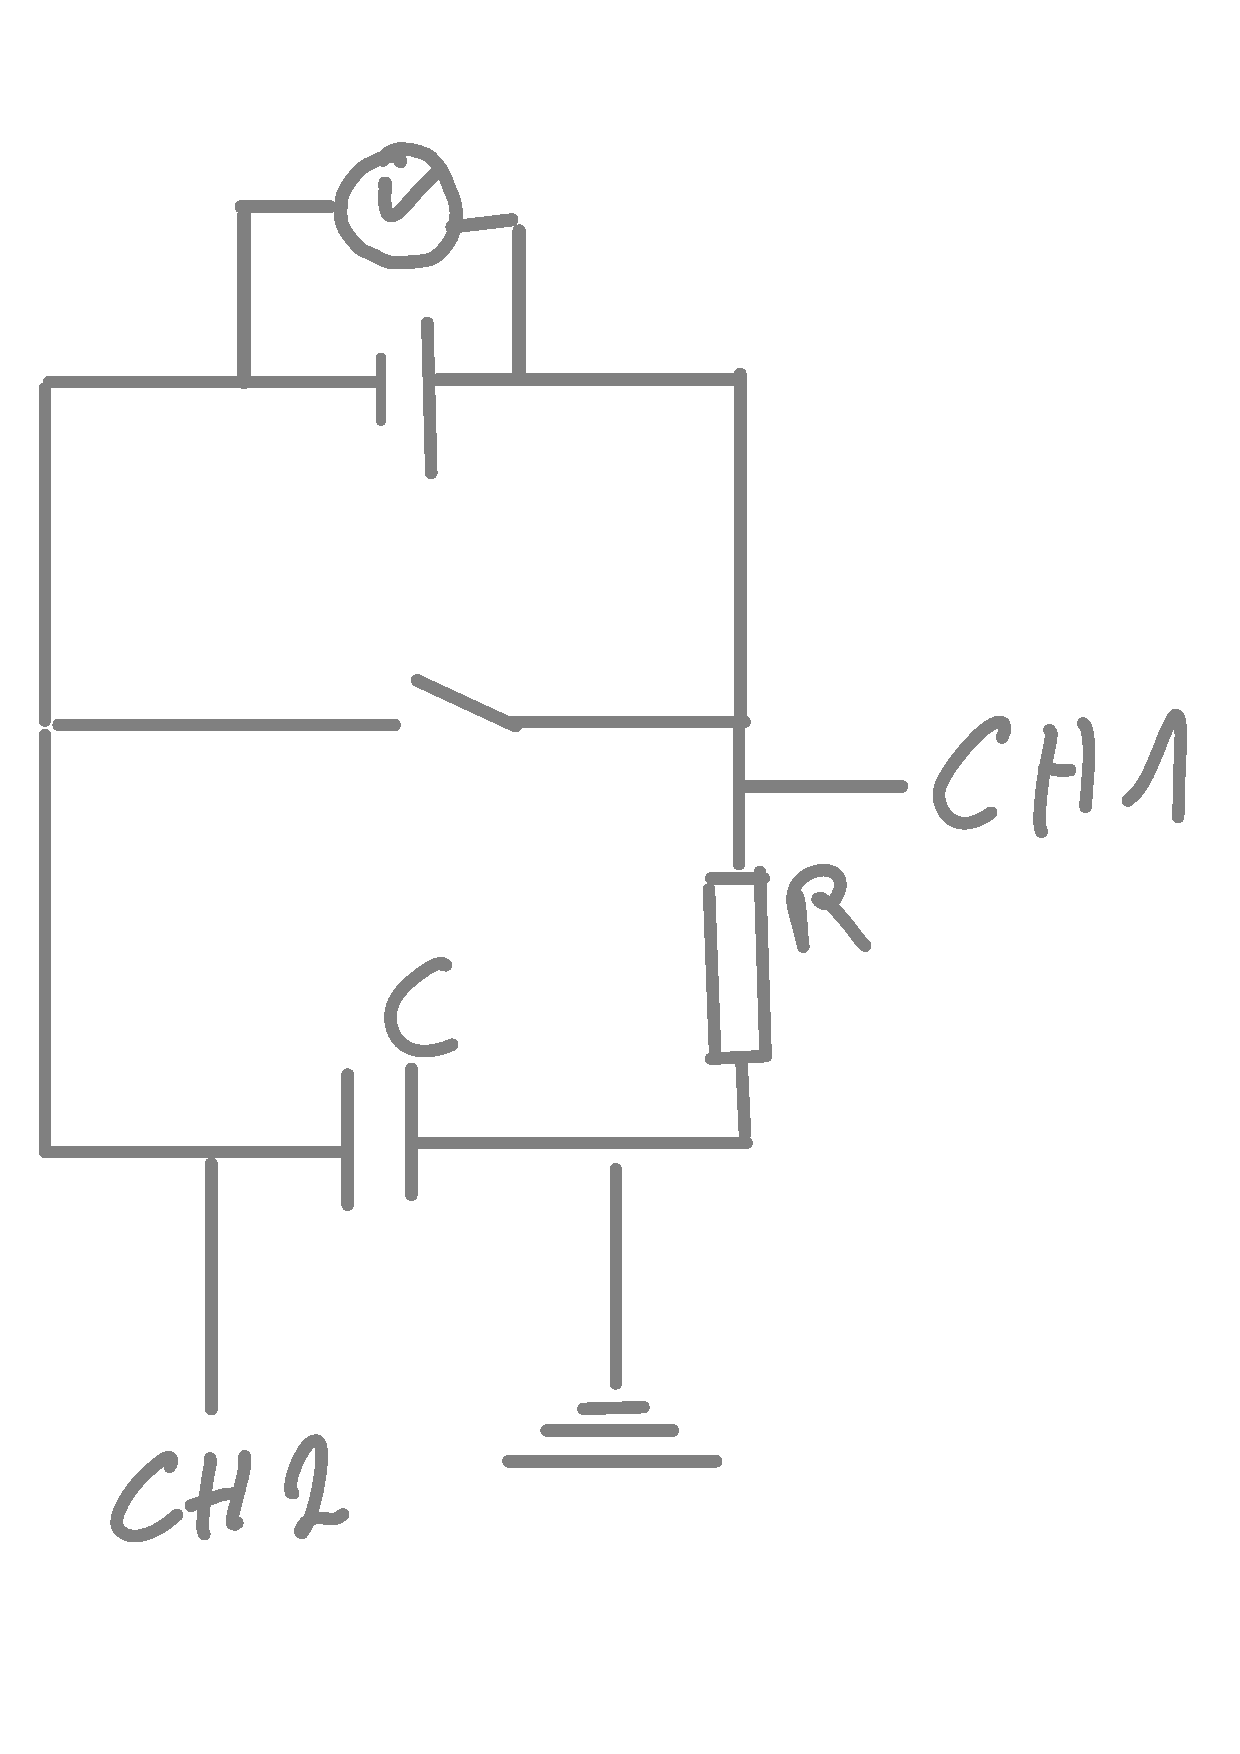
\includegraphics[width=0.5\textwidth]{schaltzkisse-osziloskop.pdf}
  \caption{Schaltplan Oszilloskop}
  \centering
  \end{figure}

  In der Obigen Skizze können Sie das Schaltbild zu dem Versuch sehen. 
  Auf dem Steckbrett werden hierfür Kondensator und Wiederstand in Reihe gesteckt.
  Parallel zu dem Kondensator wird ein Schalter eingebaut, der bei bedarf den Stromkreis
  schließen bzw. öffnen kann. Ebenfalls paralell wird eine Spannungsquelle angeschlossen. 
  Hier wird das Sensor CASSY als Spannungsquelle Verwendet. Wir haben außerdem noch mit dem
  Sensor CASSY die angelegte Spannung gemessen. An diese Schalltung muss dann noch das 
  Oszilloskop angeschlossen werden. Dieses misst gegen die gleiche Masse. Weswegen die Masse
  zwischen Kondensator und Wiederstand angeschlossen wird. Chanel 1 \& 2 werden wie im Schaltbild angeschlossen.
   So wird auf CH2 die Spannung die über den Kondensator abfällt gemessen, und 
  auf CH1 die Spannung die über den Wiederstand abfällt. 

  \begin{figure}[H]
  \centering
  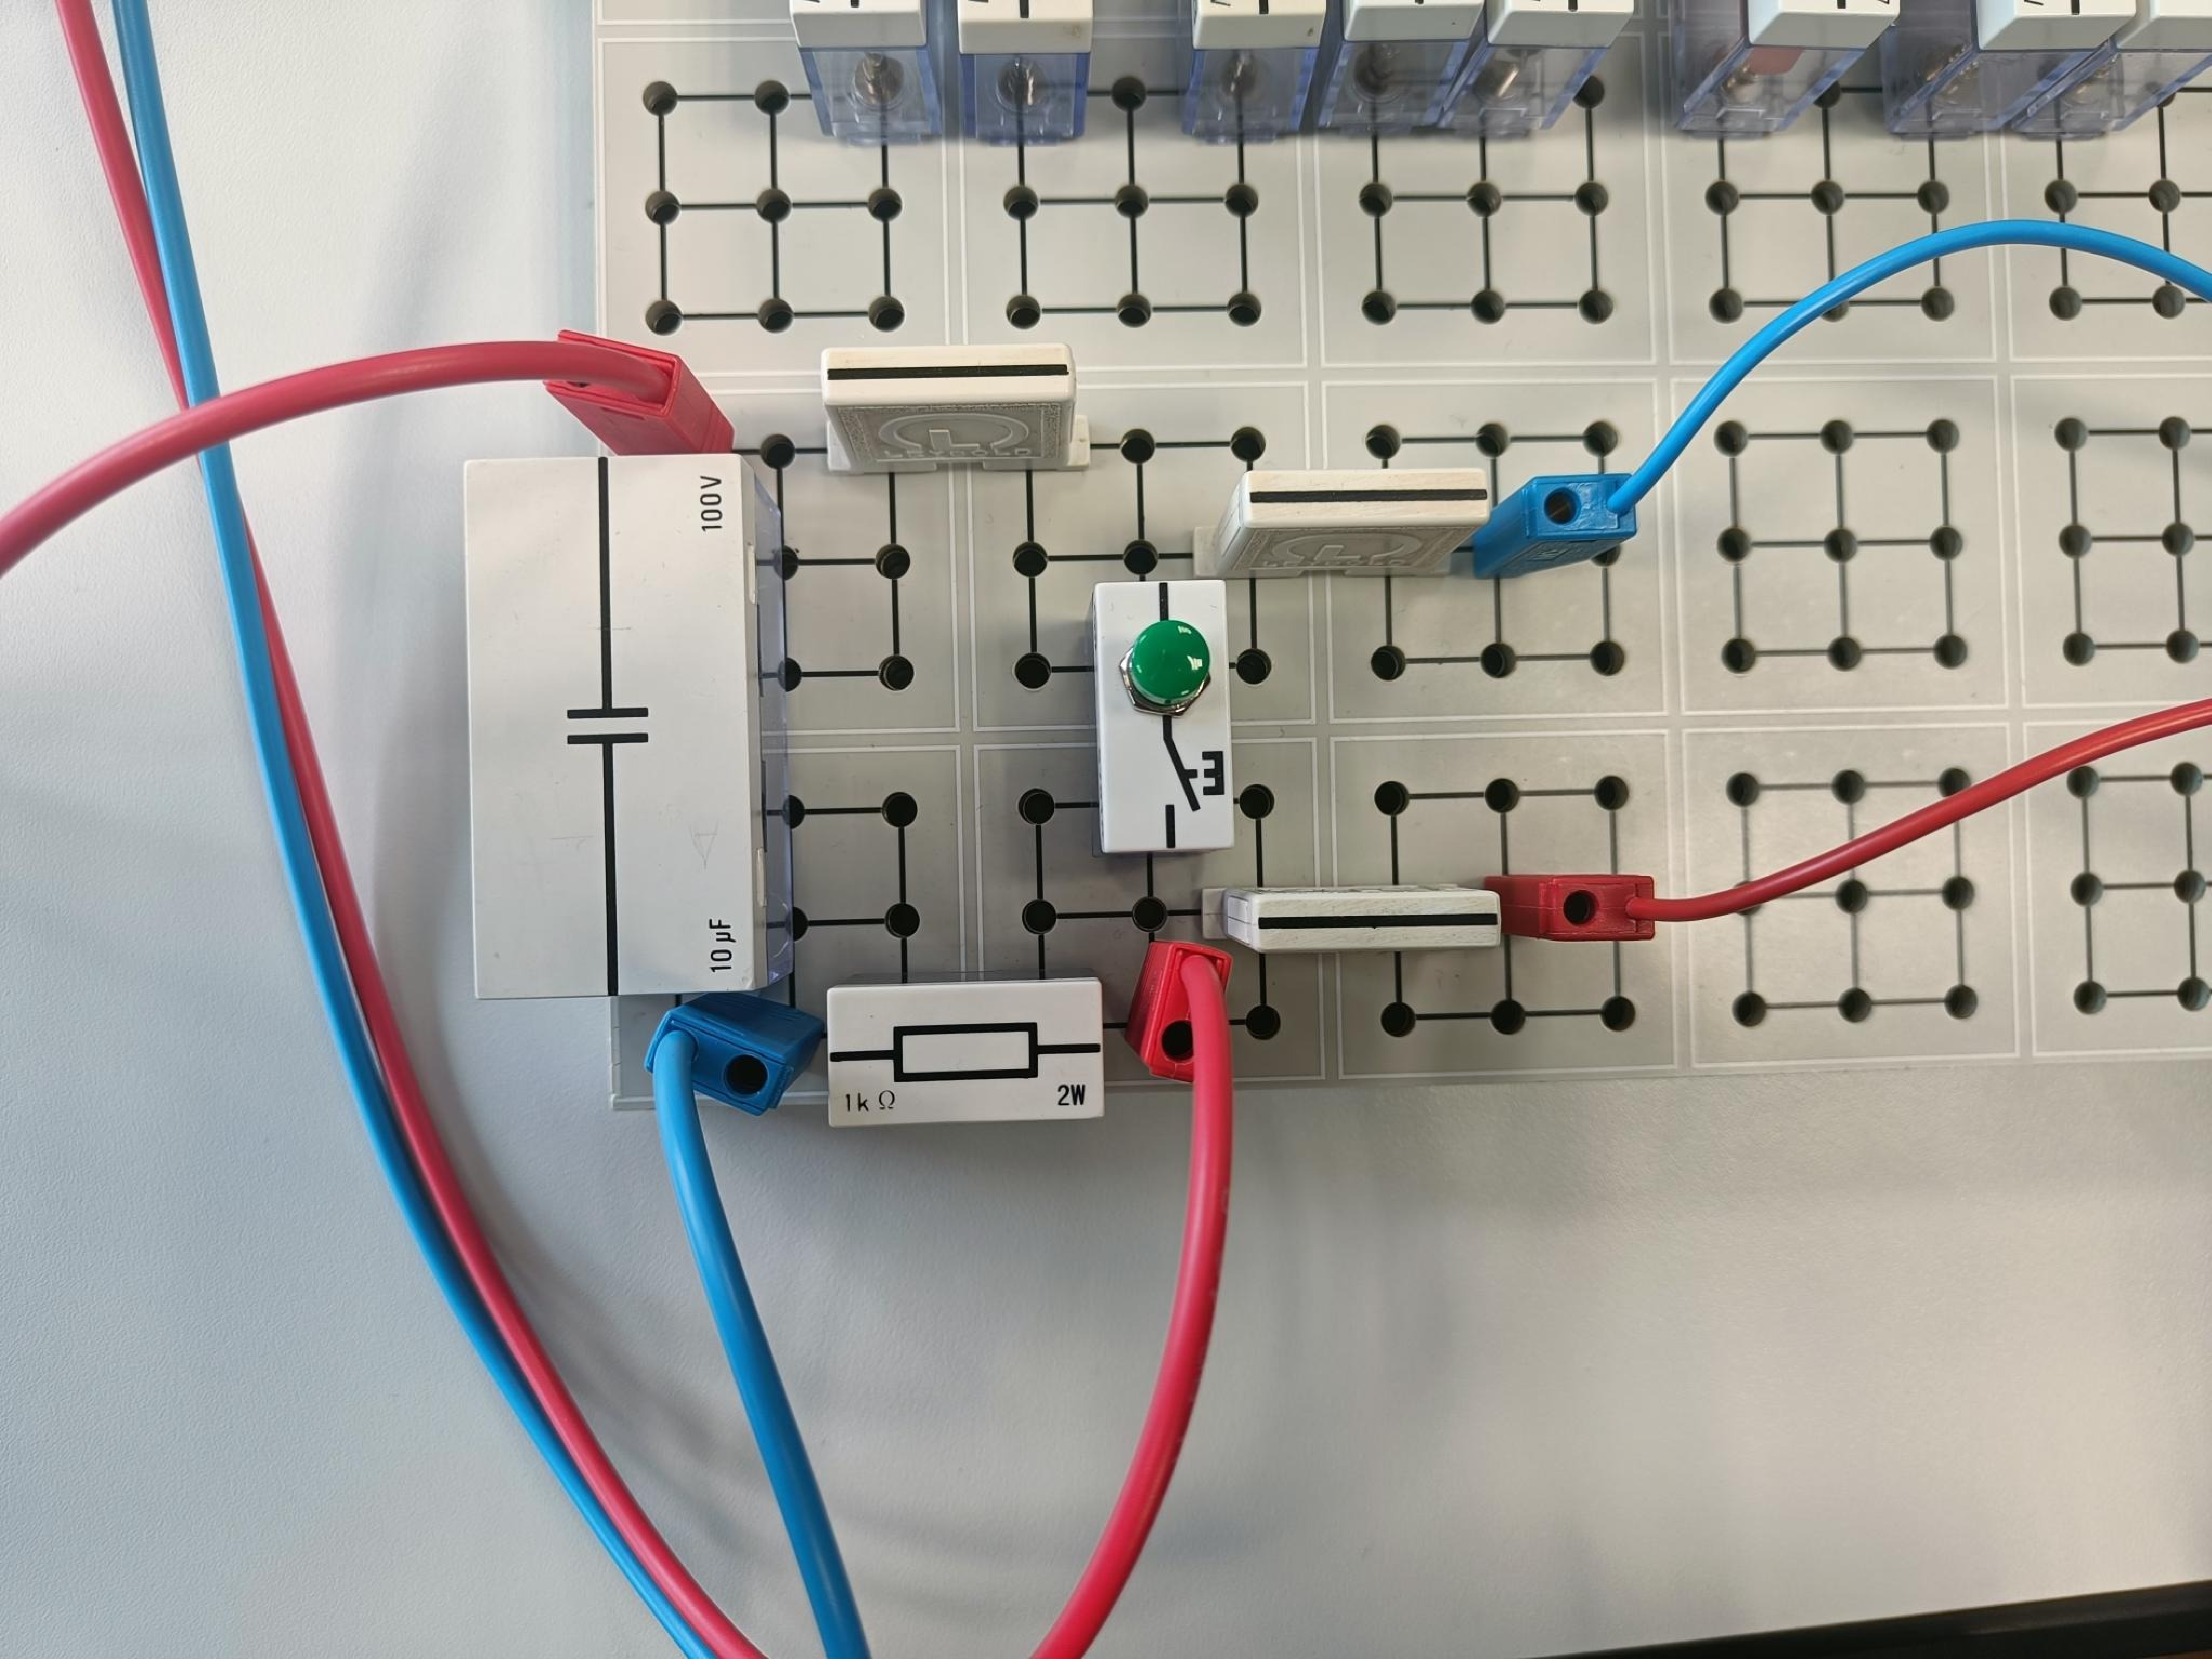
\includegraphics[width=0.5\textwidth]{Bilder_Osziloskop/Schaltung_Osziloskop_02.pdf}
  \caption{Bild der Schaltung}
  \centering
  \end{figure}
 
  Bei der Versuchsdurchführung haben wir wie im Aufbau bereits beschrieben den Versuch 
  aufgebaut. Um die Spannung ein zu stellen, und das die Auflösung des Osziloskop richtig zu
  wählen, haben wir das Sensor CASSY verwendet um die eingangsspannung zu bestimmen. Diese haben
  wir dann auf 7.11V geregelt, wobei der Wert welcher das Sensor CASSY gemessen hat leicht 
  geschwankt hat zwischen 7.11V und 7.10V. Die eingangsspannung haben wir so gewählt, 
  damit wir vom Oszilloskop den Gesamten Bildschirm ausnutzen können Zur Einstellung des     Oszilloskops haben wir zunächst die Entladung des Kondensators betrachtet. 
  Hierfür haben wir den Trigger auf CH2 auf 7.00V 
   steigende Flanke gestellt. Steigende Flanke ist hier sinnvoll, da auf Grund der Polung 
  die Spannung am Kondensator negativ ist. Somit steigt die Spannung asymtotisch zu null. 
  Zum starten der Messung haben wir den in der Schaltung verbauten Taster betätigt.
  So konnten wir eine erste entladung aufzeichnen. Hierraus konnten wir dann die Restlichen 
  Einstellungen schließen. Ziel war es, möglichst viel vom Entladevorgang auf zu zeichnen, und 
  einen kurzen Zeitraum vor dem Entladen.
  wir haben die Zeiteinstellungen so gewählt, dass 5 $\tau$ auf unserem Bildschirm angezeigt
  werden. So sind wir sicher gegangen, dass wir nur den relevanten teil der Entladung aufzeichnen, 
  und nicht die Zeitspanne in welchem die Spannungen asymtotisch gegen null streben. 

	
\begin{figure}[H]
  \centering
  \includegraphics[width=0.7\textwidth]{Bilder_Osziloskop/Triggermenü_Osziloskop.pdf}
  \caption{Triggermenü des Oszilloskops}
  \centering
\end{figure}

Oben sehen sie ein Bild des Triggermenüs des Osziloskops. Hier haben wir sämtliche Triggereinstellungen für das Messen des Entladens eingestellt gehabt. 
Hier sieht man auch, dass wir das Signal von CH2 invertiert haben, um dieses angenehmer
auf dem Bildschirm darstellen zu können. So konnten wir außerdem den Nullpunkt der beiden 
Spannungsverläufe optisch an die ungefähr gleiche Stelle legen. Der folgenden Tabelle
können sie die Einstellungen entnehmen die wir am Oszilloskop gemacht haben.
Diese Einstellungen sind spezifisch für den Entladevorgang.


\begin{table}[H]
        \centering
        \begin{tabularx}{0.8\textwidth}{X c c c c} % adjust width as needed
            \toprule
            \textbf{Chanel} & \textbf{Kästchen} & \textbf{M} & \textbf{Trigger} & \textbf{Flanke} \\
            \midrule
            CH1 & 1.00V & 5.00ms & -- & -- \\
            CH2 & 1.00V & 5.00ms & 7.00V & positiv \\
            \bottomrule
        \end{tabularx}
        \caption{Übersicht der Einstellungen am Oszilloskop}
        \label{tab:mytable}
    \end{table}

Wir haben die Messung der Entladung mit unseren neuen Einstellungen wiederholt. Um zu überprüfen ob diese passen und reproduzierbar sind. 

%TODO : Hier ofsetmessung einfügen. 

\end{aufgabe}


\begin{figure}[H]
  \centering
    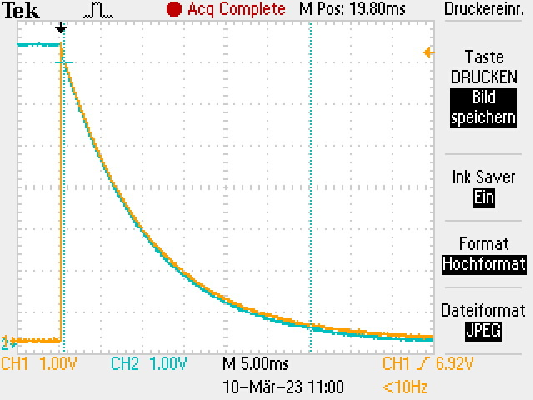
\includegraphics[width=0.7\textwidth]{Bilder_Osziloskop/Entladen_Kondensator_02.pdf}
    \caption{Endlade Vorgang vom Wiederstand und dem Kondensator}
  \centering
\end{figure}
Oben Abgebildet ist der Spannungsverlauf am Kondensator (blau) und am Wiederstand (rot) während des Entladens.
Hier ist zu beachten, das Channel 2 (der Kondensator) invertiert ist in der Darstellung.
Dies haben wir gemacht, damit wir die Nulllinien angenehm aufeinander legen können, und um einen großteil des Bildschirmes vom Oszilloskop zum ablesen verwenden zu können, um ablese Fehler zu minimieren.
Diese Entladekurven ensprechen dabei unserer erwartung, da sie in etwa nach einer exponentiellen abnahme aussehen.

Zur bestimmung von $\tau$ haben wir dann bei der Entladung insgesamt 4 Messungen durchgeführt. 
Jewails 2 für Kondensator und Wiederstand. Dies haben wir getan um zu überprüfen ob unsere Messungen reproduzierbar waren. 
Und um sicher zu gehen, dass unsere Messung kein Ausreißer war. 

Für die Messung des Aufladevorgangs mussten wir nur die Trigger einstellungen ändern sonst konnten wir unsere Einstellungen übernehmen. In diesem Fall haben wir auch keins der Signale invertiert. 

\begin{table}[H]
        \centering
        \begin{tabularx}{0.8\textwidth}{X c c c c} % adjust width as needed
            \toprule
            \textbf{Chanel} & \textbf{Kästchen} & \textbf{M} & \textbf{Trigger} & \textbf{Flanke} \\
            \midrule
            CH1 & 1.00V & 5.00ms & -- & -- \\
            CH2 & 1.00V & 5.00ms & -80.0mV & positiv \\
            \bottomrule
        \end{tabularx}
        \caption{Übersicht der Einstellungen am Oszilloskop}
        \label{tab:mytable}
    \end{table}
    
Beim messen der Aufladung haben wir zunächst denn Schalter gedrückt und auch einige Sekunden gewartet, um sicher zu gehen, dass der Kondensator entladen war. 
Dann haben wir den Schalter losgelassen un die Messung ist durch den Trigger automatisch gestartet. 
Hier haben wir ebenfalls erst eine Testmessung durchgeführt, und dann wie beim entladen jeh für Kondensator und Wiederstand 2 Messungen zur bestimmung von $\tau$ gemacht. 

\begin{figure}[H]
  \centering
    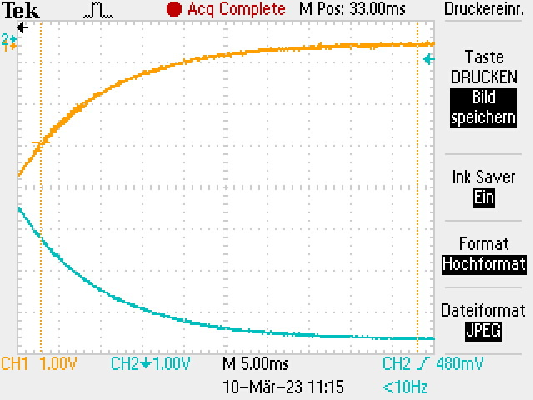
\includegraphics[width=0.7\textwidth]{Bilder_Osziloskop/Aufladen_Kondensator_02.pdf}
    \caption{Aufladen Vorgang vom Wiederstand und dem Kondensator}
  \centering
\end{figure}
Die Abbildung zeigt den Spannungsverlauf von einem typischem Aufladevorgang.
Hier haben wir nichts invertiert, da wir auch so die gleiche Nullline setzen konnten, und trotzdem das gesamte Display zum ablesen nutzen konnten.
Dabei ist allerdings zu beachten das wir die Null ans obere Ende gesetzt haben, da aufgrund von unserer Verkabelung die Spannung am Wiederstand sowie am Kondensator negativ waren, was für die Auswerung allerdings Irrelevant ist.
Auch hier entsprechen die beiden Kurven (zumindest nach Augenmaß) einer Exponentiellen abnahme im Fall der Kondendensator Spannung, bzw. einer Exponentiellen zuname für die Stromstärke.

Zur bestimmung von Tau haben wir mit dem Cursors je zwei Messwerte abgelesen. 
Mithilfe der Formeln die wir bereits in den Grundlagen eingeführt haben, konnten wir dann die Zeitkonstante bestimmen. 
Diese erhalten wir indem wir den quotienten von unserem Werte Paar nehmen und dann nach $\tau$ umformen. Daraus ergibt sich :

\begin{equation}
	\tau = \frac{t_2 - t_1}{ln\left(\frac{u_1-U_{off}}{U_2-U_{off}}\right)}	
\end{equation}

Wobei wir hier noch den möglichen Ofset beachten müssen. Die obige Formel können wir jedoch nicht für den Aufladevorgang des Kondensators verwenden, wenn wir an diesem den Spannungsabfall messen, da die Funktion die diesen beschreibt von der Form $ y = 1 - e^x $ ist. 
In diesem Fall erhalten wir für die Zeitkonstante:
 
 \begin{equation}
 other equation
\end{equation}

Somit können wir Die zeitkonstante für unsere Messungen bestimmen. Auf grund der ablesegenauigkeit kommt jedoch auf diesen noch ein Fehler. 
Diesen können wir mit statischtischer Fehlerfortplanzung bestimmen.

 
\begin{aufgabe}{Lade- und Entladekurven des Kondensators mit Cassy}
  Zeigen Sie für den Lade- und den Entladevorgang jeweils ein Bild des
  Spannungsverlaufs am Kondensator und des Lade- bzw.~Entladestroms.
  Korrigieren Sie erforderlichenfalls den Spannungs- und/oder
  Strom-Offset. Transformieren Sie die Rohdaten geeignet in
  logarithmische Größen und bestimmen Sie mittels linearer Regression
  die Zeitkonstante. Beschreiben Sie, wie Sie die Messunsicherheiten
  behandeln. Berechnen Sie das gewichtete Mittel und geben Sie Ihr
  Endergebnis für die Kapazität mit statistischer und systematischer
  Messunsicherheit an.
\end{aufgabe}


\begin{aufgabe}{Zusammenfassung und Diskussion}
  Fassen Sie Ihre Ergebnisse zu den Kapazitäten zusammen und
  vergleichen Sie sie untereinander, mit den Messungen aus dem
  Vorversuch und mit den Herstellerangaben (Toleranz
  $\SI{5}{\percent}$).  
\end{aufgabe}

 
 
 
\end{document}
